\documentclass[tikz, crop, border = {2pt 2pt 2pt 2pt}]{standalone}

\usepackage{physics}
\usetikzlibrary{decorations.pathreplacing, calligraphy}

\usepackage{concmath-otf}

\begin{document}
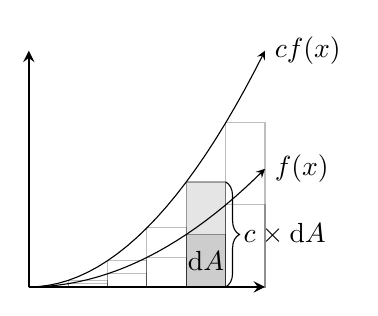
\begin{tikzpicture}
    \draw[thick, -stealth] (0, 0) -- (0, 3);
    \draw[thick, -stealth] (0, 0) -- (3, 0);

    \draw[-stealth, domain = 0:3] plot (\x, {\x*\x*1/6}) node[right]{$f(x)$};
    \draw[-stealth, domain = 0:3] plot (\x, {\x*\x*1/3}) node[right]{$cf(x)$};

    \foreach \x in {0.5, 1, 1.5, 2.0, 2.5} {
        \draw[lightgray, blend mode = multiply] (\x, 0) rectangle ++ (0.5, {\x*\x*1/6});
        \draw[lightgray, blend mode = multiply] (\x, 0) rectangle ++ (0.5, {\x*\x*1/3});
    }
    \filldraw[lightgray!40, blend mode = multiply] (2.0, 0) rectangle ++ (0.5, {4*1/3});
    \filldraw[lightgray!40, blend mode = multiply] (2.0, 0) rectangle ++ (0.5, {4*1/6}) node[midway, black]{$\dd{A}$};
    \draw[decorate, decoration = {brace, amplitude = 5pt, mirror}] (2.5, 0) -- ++ (0, {4*1/3}) node[right = 3pt, midway]{$c\times\dd{A}$};
\end{tikzpicture}
\end{document}